\documentclass[conference]{IEEEtran}

\usepackage{graphicx}
\usepackage{amsmath,amssymb}
\usepackage{booktabs}
\usepackage{tabularx}
\usepackage{array}
\usepackage{multirow}
\usepackage{xcolor}
\usepackage{url}
\usepackage{enumitem}
\usepackage{xeCJK}
\setCJKmainfont{AR PL SungtiL GB}
\setCJKmonofont{FandolFang}

\title{Red team testing for recommendation systems driven by large language models}

\author{%
\IEEEauthorblockN{Sbaaoui Idriss}
\IEEEauthorblockA{%
Student ID: 22060004\\
Department / Major: Computer Science\\
University: 华东理工大学\\
Supervisor: 张恒润
}
}

\begin{document}
\maketitle

\begin{abstract}
Large language model (LLM) modules are now used in many recommendation pipelines for retrieval, reranking, and explanation generation. This adds flexibility, but it also opens a new risk: recommendation outputs can shift when retrieval data or prompt-facing text is manipulated. This proposal presents a planned study, \emph{Red team testing for recommendation systems driven by large language models}, using Rag-Poison-Lab as the experiment platform. The study tracks how poisoning signals move from indexing and retrieval to reranking and final item exposure. The core question is simple: where does manipulation first take hold, and how far does it travel? To answer that, the plan runs controlled baseline-versus-attacked comparisons with repeatable data preparation, dual indexes, trace logs, and metric reporting that covers both recommendation quality and attack impact. The work stays at proposal stage and defines research questions, a technical plan, environment assumptions, budget and sustainability limits, and a 20-week schedule. The expected contribution is a practical red-team testing process for LLM-driven recommendation systems that can support later thesis work on robustness and reliability.
\end{abstract}

\section{Research Background}
Recommendation systems are moving from closed ranking pipelines to mixed systems that combine retrieval engines, deep ranking modules, and natural-language interfaces. In LLM-assisted settings, recommendation is no longer only a score-prediction task. It also depends on retrieval and language understanding. Users may receive recommendations through generated explanations or conversational ranking requests, and both rely on text-processing stages \cite{lewis2020rag,hou2024llmrankers}.

This shift is why this study is needed. In a traditional setup, utility metrics may be the main quality signal. In an LLM-driven retrieval pipeline, that alone is not enough. Final top-$K$ results can change because candidate evidence changes, reranking context changes, or adversarial payload text appears at the wrong stage. For that reason, this proposal treats the recommender as a \emph{pipeline under adversarial pressure}, not just a single model.

Red-team testing is a good response. Instead of assuming benign inputs, it defines attacker goals and limits first, then tests whether the system remains stable. In recommendation tasks, this allows planned evaluation of targeted promotion, poisoned exposure, ranking instability, and explanation-level influence under controlled conditions.

In this proposal, I use Rag-Poison-Lab because it already supports the core controls needed for this work: deterministic preprocessing, attack-profile configuration, baseline/attacked indexing, recommendation serving, trace extraction, and report generation \cite{ragpoisonlab2026}. The goal is not to present a finished security framework. The goal is to use this platform as a practical base for a clear proposal-stage study.

The broader motivation is reliability in AI-based choice systems. Recommendation outputs influence what users watch, read, and buy. If adversarial text consistently pushes those outputs, the issue is both technical and practical. A movie can climb a list for the wrong reason. This is why the proposed work focuses on a controlled evaluation workflow with clear evidence instead of informal attack demos.

\subsection{Fundamentals of Deep Learning}
Deep learning matters in this proposal because recommendation quality now depends on learned representations across multiple data types. User interactions, item metadata, and text fields are mapped into latent spaces where ranking decisions are made \cite{lecun2015deep}. This is useful, but it also means that small input changes can travel through the system in ways that are hard to see directly.

Three fundamentals are especially important for the planned study. First, embedding space structure shapes ranking outcomes: small shifts in representation can change candidate neighborhoods and recommendation order. Second, deep systems are sensitive to distribution shift, so strong benign performance does not guarantee stable behavior under poisoned corpora. Third, in LLM-assisted recommenders, behavior is spread across retrieval, reranking, and explanation stages. So the analysis should check each stage.

These fundamentals directly shape the proposal design. The study aims to preserve utility under benign settings, measure quality drops under adversarial settings, and identify where perturbations become strongest along the pipeline. This suggests that evaluation method matters as much as model choice. The contribution is mainly in evaluation method, not new model design: this project does not claim a new deep model, but proposes a controlled way to evaluate robustness behavior in an existing recommendation stack.

Another practical point is resource limits. Retrieval depth, reranking mode, and batch scope affect both results and cost. The proposed workflow uses fixed experiment grids and clear run snapshots so that observed differences come from attack conditions, not hidden setting changes.

Finally, this section treats deep learning as something to analyze, not a black box. The study will interpret metric shifts with trace evidence whenever possible. This keeps the final thesis argument clearer and more credible.

\subsection{Neural Network}
Neural networks provide core modeling tools for both recommendation ranking and language-based reasoning. Feed-forward layers, embedding modules, and transformer-style architectures map mixed inputs into ranking signals. Prior neural collaborative filtering work showed why this matters: user-item interactions can be modeled beyond linear assumptions, improving expressive power \cite{he2017ncf}.

In this proposal, neural-network relevance appears in four practical aspects:

\begin{enumerate}[leftmargin=*]
\item \textbf{Representation learning}: user preference context and item semantics are represented in latent spaces where nearest-neighbor and ranking decisions are computed.
\item \textbf{Nonlinear ranking behavior}: small input shifts can produce nontrivial output reordering, especially in reranking steps.
\item \textbf{Prompt-conditioned reasoning}: LLM reranking and explanation are generation processes sensitive to context framing.
\item \textbf{Compositional vulnerability}: vulnerabilities can emerge at inter-module boundaries rather than from a single neural block.
\end{enumerate}

A key assumption in this proposal is that capability and robustness should be evaluated separately. A network can be expressive but still vulnerable under adversarially modified retrieval inputs. For that reason, I prioritize controlled baseline-attacked comparison over clean-data accuracy alone.

The project further separates \emph{model-internal} and \emph{pipeline-external} causes of ranking change. Model-internal causes refer to learned scoring behavior under stable inputs. Pipeline-external causes include manipulated retrieval records and prompt-facing payload fields that alter candidate pools before final scoring. This distinction is needed if the final analysis is expected to support practical security recommendations.

In addition, the thesis will analyze explanation outputs as part of neural behavior. Explanations are not only interface text. They also influence trust and perceived relevance. If poisoned evidence changes explanation generation, the risk extends from ranking quality to user persuasion. The study treats explanation quality and consistency as an additional robustness concern.

\subsection{Retrieval-Augmented Generation and Ranking Pipeline}
The core of this proposal is a retrieval-augmented recommendation workflow with explicit baseline and attacked branches. This choice is deliberate: the research question is about how adversarial influence moves through a full pipeline, not just one model component. Based on local audit, Rag-Poison-Lab already provides the needed setup---deterministic preprocessing, dual-index management, retrieval and ranking control, trace export, and evaluation scripts \cite{ragpoisonlab2026}. So the platform fit is practical, not theoretical.

Figures~\ref{fig:architecture} and~\ref{fig:workflow} summarize the planned experiment setup. In the thesis workflow, this architecture will be treated as a controlled plan: same user/query conditions, same output interface, and different index conditions.

\begin{figure}[t]
    \centering
    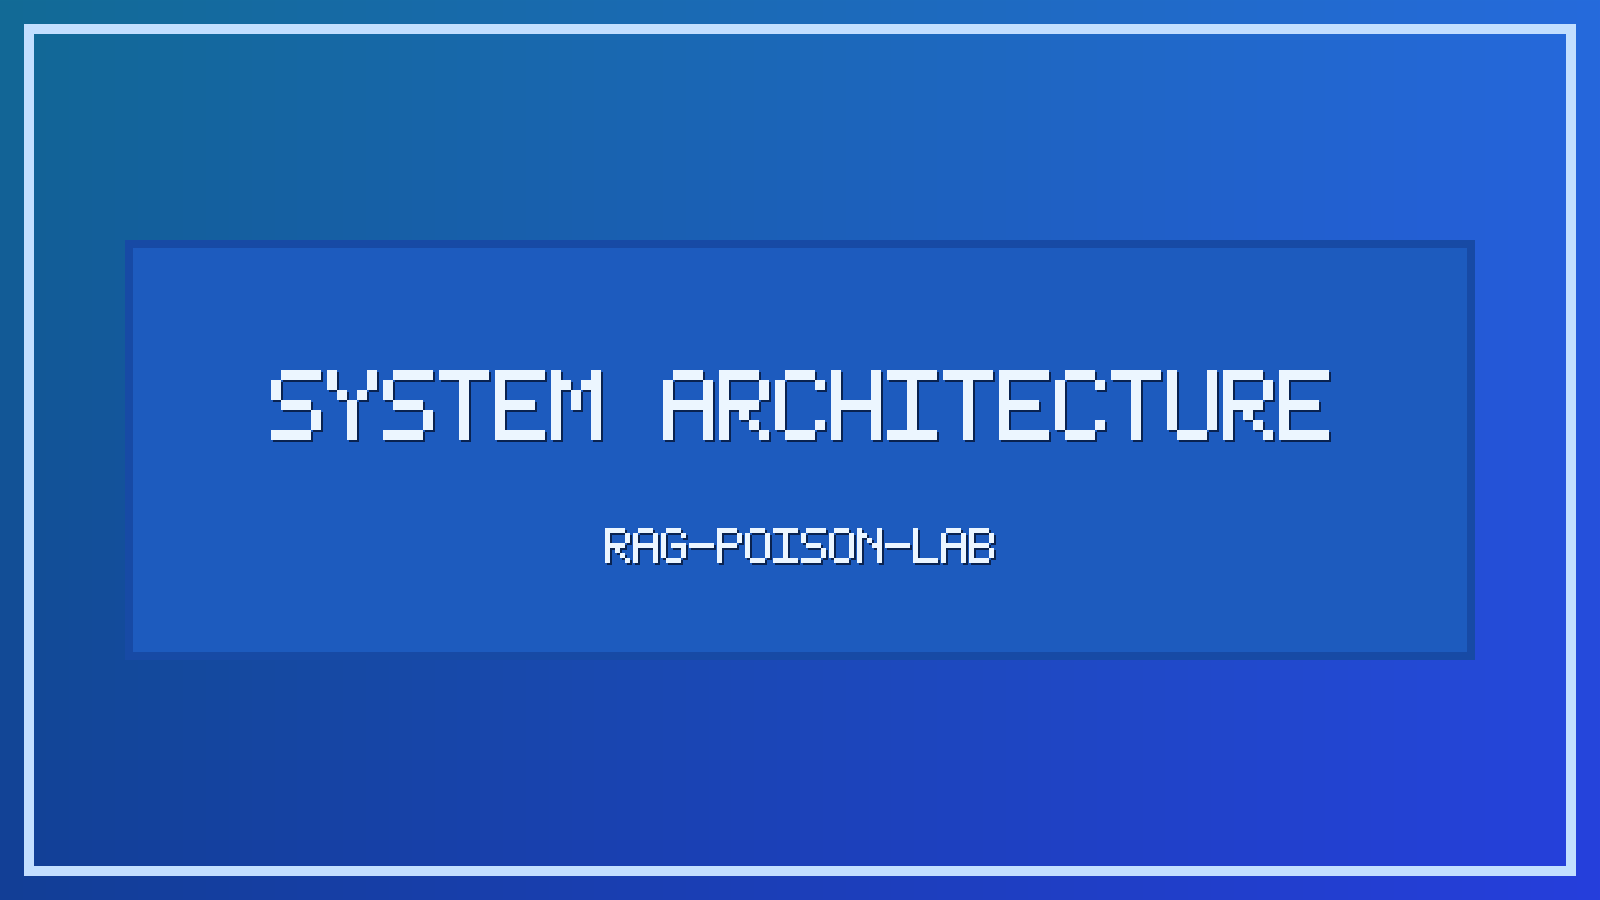
\includegraphics[width=0.98\columnwidth]{figures/architecture_placeholder.png}
    \caption{Planned overall architecture of the Rag-Poison-Lab red-team evaluation platform.}
    \label{fig:architecture}
\end{figure}

\begin{figure}[t]
    \centering
    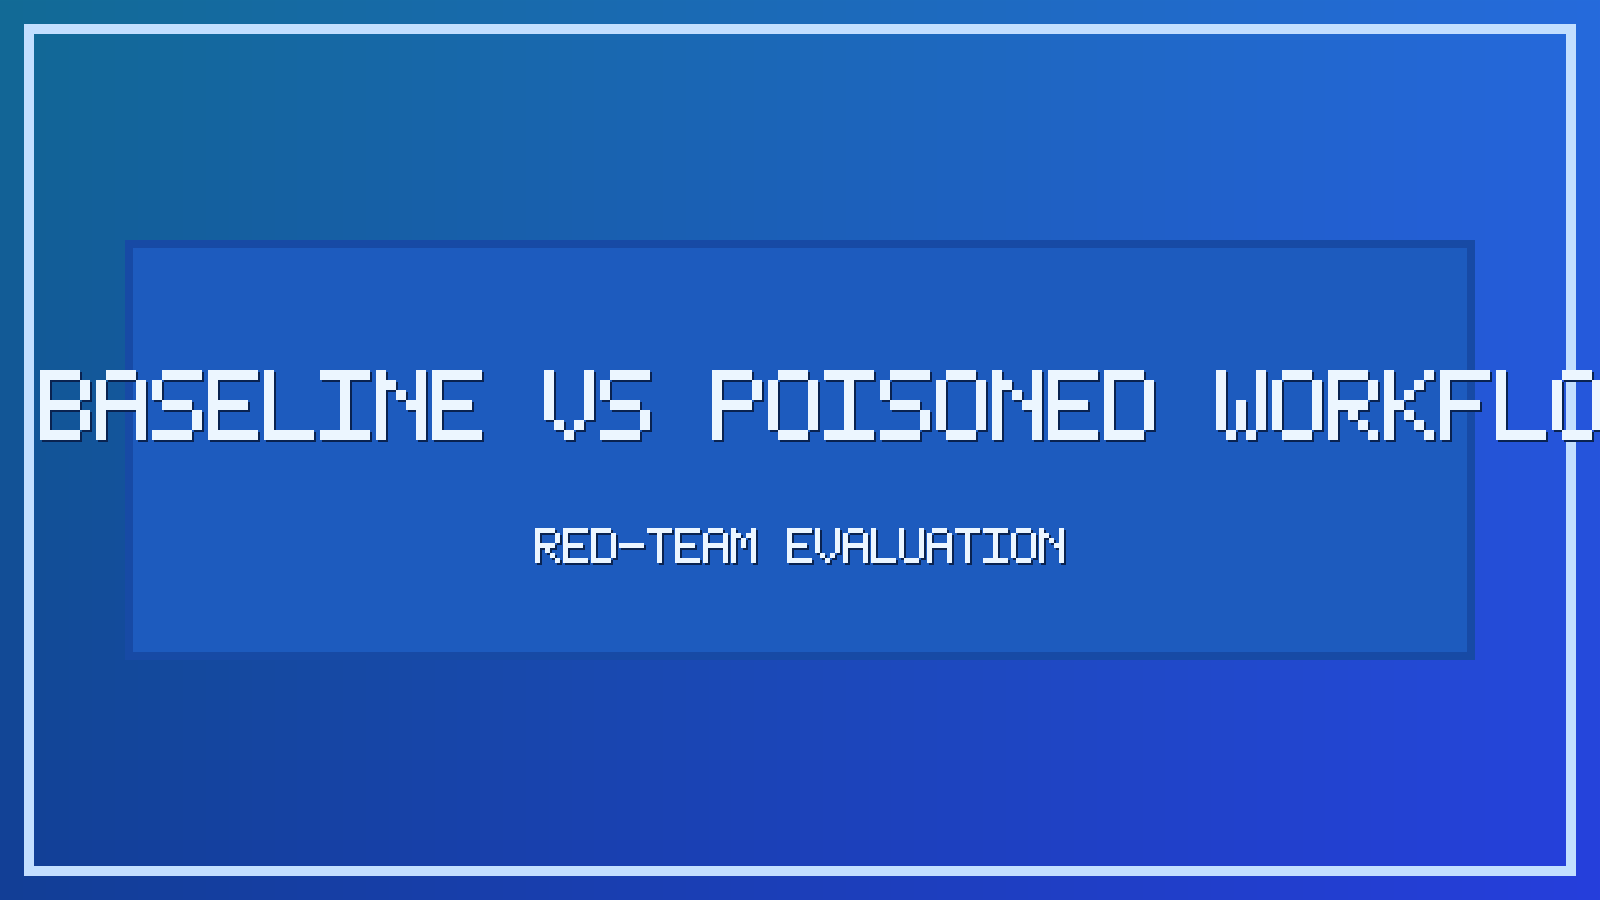
\includegraphics[width=0.98\columnwidth]{figures/workflow_placeholder.png}
    \caption{Planned baseline-versus-poisoned workflow for controlled adversarial comparison.}
    \label{fig:workflow}
\end{figure}

\begin{table}[t]
\caption{Planned pipeline stages and observable artifacts}
\label{tab:pipelinestages}
\centering
\begin{tabularx}{\columnwidth}{>{\raggedright\arraybackslash}p{0.23\columnwidth} >{\raggedright\arraybackslash}X}
\toprule
Stage & Planned observable outputs \\
\midrule
Data preparation & Processed movie/rating/split/profile files; deterministic hashes \\
Attack preparation & Attack configuration snapshots; poisoned bulk metadata \\
Indexing & Baseline index and attacked index with aligned mappings \\
Retrieval & Retrieval query text; candidate list; poison marker visibility \\
Ranking / reranking & Top-$K$ list, score signals, rerank prompt/response traces \\
Explanation path & One-sentence explanations per item with mode context \\
Evaluation & Utility metrics, attack metrics, per-user deltas, aggregated reports \\
\bottomrule
\end{tabularx}
\end{table}

Retrieval is not treated as only a preprocessing step in this proposal. It is an active factor in robustness. If ranking is the visible output, retrieval is the gate that decides what can be seen. Candidate generation relies on BM25-style search over title, genre, and synopsis fields \cite{robertson2009bm25}; poisoning in those fields can change the candidate pool before ranking starts.

The proposed pipeline design includes two controls:
\begin{itemize}[leftmargin=*]
\item \textbf{Mode control}: identical user/query settings are evaluated across baseline and attacked indexes.
\item \textbf{Trace control}: retrieval evidence and reranking artifacts are recorded to support later analysis of where changes came from.
\end{itemize}

That setup lets the study ask not only \emph{whether} outputs change, but also \emph{where} and \emph{why} the change appears along the pipeline. That distinction is central to this proposal.

\subsection*{Planned Data and Index Rules}
To keep adversarial effects easy to interpret, the proposal introduces clear data and index rules. First, baseline and attacked indexes will share schema, mapping design, and retrieval settings; this avoids mixed effects from structure differences. Second, each attacked-index build will include metadata snapshots (attack type, poison fraction, source hash, output hash) to keep source tracking and repeatability.

The study also proposes deterministic data processing from raw interactions to processed artifacts. This matters because adversarial effects should be compared against a stable baseline. If split logic or preprocessing settings change between runs, baseline-attacked differences become difficult to interpret. Fixed preprocessing parameters and explicit run labels are part of the planned protocol.

For retrieval rules, query formulation policy will be fixed in paired baseline-attacked comparisons. User-context construction (top genres and liked titles), retrieval depth, and seen-item filtering will stay constant---unless a specific follow-up test targets one of these factors. This isolates attack effects from query-generation variance.

Finally, trace logging is treated as mandatory. For each evaluated mode, logs will keep retrieval query text, retrieved-document summaries, poison-marker visibility, and rerank context payloads when applicable. This keeps interpretation tied to evidence instead of score-only comparison.

\section{Related Work}
This proposal draws from four literature strands: neural recommendation, recommender poisoning, retrieval-augmented generation security, and LLM-based ranking.

\subsection{Recommendation and Neural Ranking Foundations}
Pairwise ranking and neural recommendation literature established strong baselines for recommendation with implicit feedback \cite{rendle2012bpr,he2017ncf}. These works remain the right utility reference point for this thesis because robustness evaluation only matters if benign ranking quality stays acceptable.

\subsection{Poisoning and Adversarial Manipulation in Recommenders}
Adversarial research has shown that recommendation behavior can be manipulated through injected or crafted data. Poisoning attacks on factorization-based collaborative filtering demonstrated both targeted attacks and broad quality drops \cite{li2016poisoncf}. Graph-based recommender poisoning further showed that attack effectiveness can remain high even with structural constraints \cite{fang2018graphpoison}. Together, these findings support clear attacker modeling and limited perturbation budgets in this proposal.

This proposal extends that perspective to retrieval-augmented LLM recommendation settings. Instead of attacking interaction data alone, the planned experiments focus on manipulations in retrieval corpora and prompt-facing fields, where text artifacts can influence both ranking and generated explanations. That is the gap this thesis targets.

\subsection{RAG and LLM Security Literature}
RAG systems combine external retrieval with generation to improve context use and factual grounding \cite{lewis2020rag}. The same design also introduces corpus-integrity risks. Recent work reports vulnerability to retrieval poisoning and indirect prompt injection, where malicious external text alters downstream model behavior \cite{greshake2023prompt,poisonedrag2024,badrag2024}. This risk maps directly to recommendation pipelines that expose textual item fields to reranking models.

The planned study differs from general RAG security evaluation by focusing on recommendation outcomes and exposure effects. The central question is not answer correctness. It is ranking stability under adversarial retrieval conditions.

\subsection{LLMs as Rankers and Recommender Components}
Emerging evidence suggests that LLMs can function as zero-shot rankers for recommendation tasks \cite{hou2024llmrankers}. This is attractive because it reduces dependence on task-specific fine-tuning, but it also implies that ranking logic can be sensitive to subtle textual manipulation. For this reason, the proposal treats LLM reranking as a strong attack surface that should be tested under controlled red-team settings. Useful, but risky.

\subsection{Dataset and Evaluation Context}
MovieLens remains a widely used benchmark family for recommender research, with strong reproducibility value and clear historical context \cite{harper2015movielens}. For ranking metrics, established information-retrieval concepts (for example, NDCG and rank-sensitive relevance analysis) provide the baseline method \cite{manning2008ir}. This proposal keeps that combination intentionally: it grounds the study in familiar recommender and IR practice before adding poisoning-specific evaluation layers.

\begin{table*}[t]
\caption{Literature positioning for the proposed study}
\label{tab:litposition}
\centering
\begin{tabularx}{\textwidth}{>{\raggedright\arraybackslash}p{0.22\textwidth} >{\raggedright\arraybackslash}p{0.22\textwidth} >{\raggedright\arraybackslash}p{0.25\textwidth} >{\raggedright\arraybackslash}X}
\toprule
Theme & Representative references & Main contribution trend & Gap addressed by this proposal \\
\midrule
Neural recommendation baselines & \cite{rendle2012bpr,he2017ncf} & Ranking quality optimization under implicit feedback and neural interaction modeling & Limited emphasis on retrieval-corpus adversarial channels in LLM-driven stacks \\
Classical recommender poisoning & \cite{li2016poisoncf,fang2018graphpoison} & Demonstrates manipulability of recommendation outcomes through injected data or structure perturbation & Does not directly model RAG-style retrieval + LLM reranking pipelines \\
RAG and prompt security & \cite{lewis2020rag,greshake2023prompt,poisonedrag2024,badrag2024} & Shows retrieval dependency benefits and vulnerability to corpus/prompt attacks in LLM systems & Typically centers QA/chat tasks rather than recommendation exposure and ranking stability \\
LLM ranking in recommenders & \cite{hou2024llmrankers} & Establishes LLM feasibility for ranking tasks with low-shot or zero-shot setup & Requires dedicated robustness evaluation under poisoning-aware recommendation experiments \\
Evaluation and benchmark context & \cite{harper2015movielens,manning2008ir} & Provides reproducible dataset baseline and rank-sensitive evaluation foundations & Needs integration with attack metrics and traceability in one unified protocol \\
\bottomrule
\end{tabularx}
\end{table*}

Table~\ref{tab:litposition} shows the gap addressed by this proposal: prior work is strong either on recommendation poisoning or on RAG/LLM security, but fewer studies connect both in one reproducible recommendation-focused protocol. This thesis does not try to replace model-centered advances. It focuses on improving how hybrid retrieval-generation recommendation systems are measured.

\section{Technical Route}
The technical route is designed for reproducible adversarial experiments rather than one-off attack demonstrations. The guiding choice is simple: enforce baseline-attacked matching controls, structured logs, and fixed stages so each comparison stays interpretable. Clear controls first, then scale.

\subsection{Research Questions and Hypotheses}
This study proposes the following research questions (RQs):

\textbf{RQ1}: How strongly do retrieval-corpus poisoning strategies alter top-$K$ recommendation outputs in LLM-assisted recommendation pipelines?

\textbf{RQ2}: How does ranking mode (deterministic vs. LLM rerank) influence robustness under identical attack budgets?

\textbf{RQ3}: Which trace-level signals best explain utility-robustness trade-offs across baseline and attacked runs?

The corresponding working hypotheses are:
\begin{itemize}[leftmargin=*]
\item \textbf{H1}: Attacked indexes will increase poisoned or target-item exposure relative to baseline.
\item \textbf{H2}: LLM reranking will provide semantic flexibility but may amplify susceptibility to poisoned textual cues.
\item \textbf{H3}: Trace visibility (retrieved evidence + rerank context) will reduce ambiguity in interpreting attack effects.
\end{itemize}

These hypotheses are intentionally framed to be testable within the current platform design. They define a research direction, not predetermined outcomes.
Not predictions. They also determine the order of the experimental route that follows.

\subsection{Threat Model and Experimental Factors}
The project adopts a limited attacker model:
\begin{itemize}[leftmargin=*]
\item Attacker can manipulate a controlled fraction of indexed item records.
\item Attacker cannot directly alter held-out test relevance labels.
\item Attack channels include payload insertion and textual-field poisoning.
\item Attack objective can be targeted promotion or untargeted quality degradation.
\end{itemize}

Planned experimental factors include poison fraction, target selection policy, retrieval depth, ranking mode, and top-$K$ cutoff. Each run will store configuration and metadata snapshots for reproducibility and later audit. That way, when results diverge, the reason is easier to trace.

\begin{figure}[t]
    \centering
    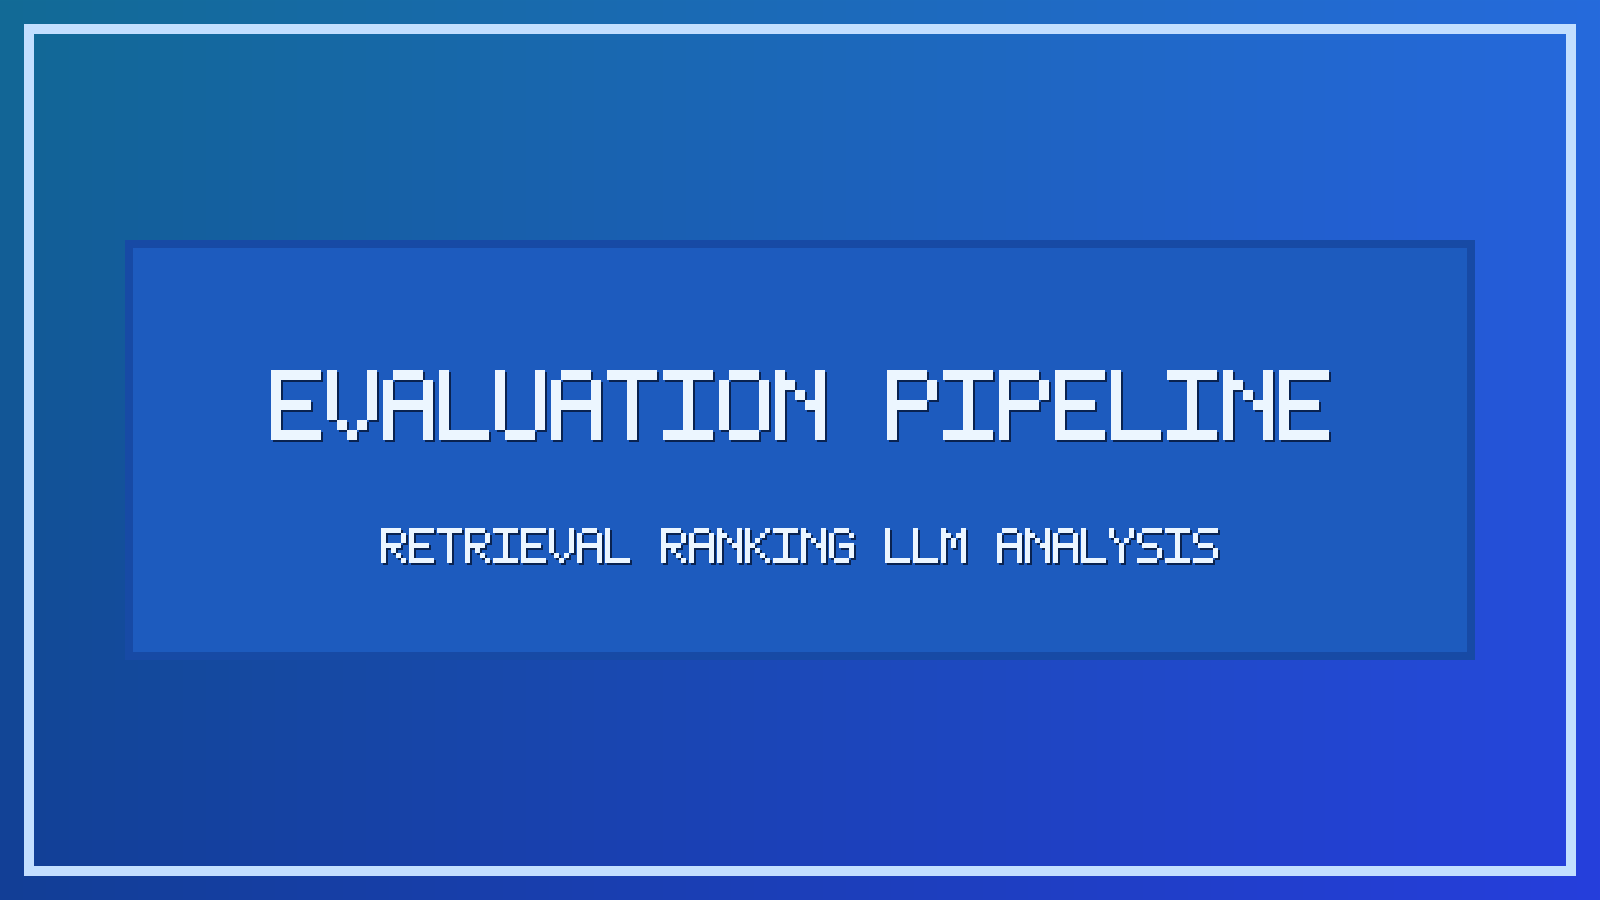
\includegraphics[width=0.98\columnwidth]{figures/evaluation_pipeline_placeholder.png}
    \caption{Planned experiment flow from preprocessing and dual indexing to trace-driven robustness analysis.}
    \label{fig:evaluationpipeline}
\end{figure}

\subsection{Execution Workflow}
The planned workflow is:
\begin{enumerate}[leftmargin=*]
\item Prepare deterministic dataset artifacts and user profiles.
\item Build baseline and attacked bulk files using fixed attack config.
\item Index both corpora under aligned schemas.
\item Run recommendation inference for selected user sets under both modes.
\item Collect traces (retrieval query, retrieved docs, rerank context).
\item Compute metric suite and aggregate deltas.
\item Generate reproducibility reports and summary artifacts.
\end{enumerate}

This route keeps interpretation clear while keeping execution complexity realistic for a graduation timeline. Simple in wording, but demanding in practice.

\subsection*{Planned Experiment Matrix}
To keep coverage broad but manageable, the proposal defines an experiment matrix that combines attack type, poison fraction, ranking mode, and evaluation scope. The matrix is organized to narrow key questions step by step:
\begin{itemize}[leftmargin=*]
\item How does attack intensity affect utility degradation and target exposure?
\item Does LLM reranking amplify or dampen attack effects under identical retrieval candidates?
\item Which conditions produce the largest baseline-attacked divergence in top-$K$ recommendations?
\end{itemize}

Experiments are planned in stages: pilot matrix (small user set), core matrix (primary batch), and sensitivity matrix (focused follow-up tests). This step-by-step plan balances statistical coverage with compute limits.

\begin{table*}[t]
\caption{Planned red-team experiment matrix (proposal stage)}
\label{tab:expmatrix}
\centering
\begin{tabularx}{\textwidth}{>{\raggedright\arraybackslash}p{0.13\textwidth} >{\raggedright\arraybackslash}p{0.14\textwidth} >{\raggedright\arraybackslash}p{0.14\textwidth} >{\raggedright\arraybackslash}p{0.12\textwidth} >{\raggedright\arraybackslash}p{0.11\textwidth} >{\raggedright\arraybackslash}X}
\toprule
Stage & Attack type & Poison fraction plan & Ranking mode & User scope & Main measurement objective \\
\midrule
Pilot A & Prompt injection & 0.01, 0.05 & Deterministic & Single + small batch & Validate pipeline integrity and trace completeness \\
Pilot B & Targeted promotion & 0.01, 0.05 & Deterministic & Small batch & Verify ASR@K and target-rank-lift computation \\
Pilot C & Prompt injection & 0.05 & LLM rerank & Small batch & Compare rerank sensitivity to poisoned payload context \\
Core 1 & Prompt injection & 0.05, 0.10, 0.20 & Deterministic + LLM rerank & Batch mode & Measure utility-robustness tradeoff under increasing attack intensity \\
Core 2 & Targeted promotion & 0.05, 0.10, 0.20 & Deterministic + LLM rerank & Batch mode & Measure targeted exposure behavior and ASR shifts \\
Core 3 & Untargeted degradation & 0.05, 0.10, 0.20 & Deterministic + LLM rerank & Batch mode & Measure broad relevance degradation and ranking instability \\
Sensitivity 1 & Prompt injection & fixed at 0.10 & Deterministic + LLM rerank & Batch mode & Vary retrieval depth and inspect candidate contamination effects \\
Sensitivity 2 & Targeted promotion & fixed at 0.10 & Deterministic + LLM rerank & Batch mode & Vary target policy and assess robustness consistency \\
Sensitivity 3 & Mixed profile stress test & fixed at 0.10 & Deterministic + LLM rerank & Full mode (limited) & Study worst-case pipeline behavior under combined perturbations \\
\bottomrule
\end{tabularx}
\end{table*}

\subsection*{Trace Analysis Protocol}
The proposal treats trace analysis as a first-class method, not a debugging afterthought. For each paired baseline-attacked run, trace comparison follows three layers:
\begin{enumerate}[leftmargin=*]
\item \textbf{Retrieval layer}: query text, candidate composition, and poisoned field visibility.
\item \textbf{Ranking layer}: score ordering changes, rerank candidate selection, and fallback behavior if applicable.
\item \textbf{Output layer}: final top-$K$ differences, explanation consistency, and target-item exposure movement.
\end{enumerate}

This layered protocol is intended to answer a central question: does performance shift originate mainly in candidate retrieval, in reranking decisions, or in both. Representative trace cases will be reported for each attack profile to complement aggregate statistics. Numbers show what moved; traces help explain why.

\subsection*{Reproducibility and Run-Output Policy}
The project proposes strict run-output management so each experiment can be reconstructed later. Planned output classes are:
\begin{itemize}[leftmargin=*]
\item run-level metric JSON summaries;
\item trace payloads for single-user deep-dive runs;
\item attack and LLM configuration snapshots;
\item markdown and CSV report outputs for comparison.
\end{itemize}

All outputs will be tagged by run label and timestamp. When possible, file hashes for core inputs (baseline and attacked bulk files) will be recorded for source checks. Plainly, every major claim should map to a concrete run output.

\subsection{Accuracy}
Accuracy in this proposal is intentionally dual-objective: \emph{recommendation utility} and \emph{attack impact}. This split is important because a system can preserve utility while still becoming easy to manipulate. Utility metrics include Precision@K, Recall@K, HR@K, MRR@K, and NDCG@K \cite{manning2008ir}. Attack metrics include ASR@K, poisoned-item exposure rate, and baseline-attacked overlap shift. In short, good ranking alone is not enough.

Let $R_u^K$ denote top-$K$ recommendations for user $u$, and let $G_u$ denote relevant held-out items. The proposal uses:
\begin{align}
\mathrm{Precision@K}(u) &= \frac{|R_u^K \cap G_u|}{K}, \\
\mathrm{Recall@K}(u) &= \frac{|R_u^K \cap G_u|}{|G_u|}, \\
\mathrm{HR@K}(u) &= \mathbb{1}\left(|R_u^K \cap G_u| > 0\right).
\end{align}

For rank sensitivity:
\begin{equation}
\mathrm{NDCG@K}(u) = \frac{1}{\mathrm{IDCG@K}(u)}\sum_{r=1}^{K}\frac{\mathrm{rel}_{u,r}}{\log_2(r+1)}.
\end{equation}

For attack success under targeted promotion:
\begin{equation}
\mathrm{ASR@K} = \frac{1}{|U|}\sum_{u \in U}\mathbb{1}(t \in R_u^K),
\end{equation}
where $t$ is the attack target item.

To characterize poisoning visibility in outputs, the proposal also defines:
\begin{equation}
\mathrm{PER@K} = \frac{1}{|U|}\sum_{u \in U}\frac{|P \cap R_u^K|}{K},
\end{equation}
where $P$ is the set of poisoned items.

The study will report per-user metrics, overall summaries, and baseline-attacked deltas. Confidence intervals will be estimated through repeated runs or bootstrap resampling when feasible. This reduces over-interpretation of single-run variation. Within this design, metric reporting is not only descriptive; it is part of the robustness argument.

\begin{table}[t]
\caption{Planned metric interpretation map}
\label{tab:metricmap}
\centering
\begin{tabularx}{\columnwidth}{>{\raggedright\arraybackslash}p{0.24\columnwidth} >{\raggedright\arraybackslash}X}
\toprule
Metric & Interpretation objective \\
\midrule
Precision@K, Recall@K & Utility quality at recommendation cutoff \\
HR@K, MRR@K & Hit sensitivity and early-rank relevance behavior \\
NDCG@K & Position-sensitive relevance with logarithmic discount \\
ASR@K & Targeted attack effectiveness on exposure outcomes \\
Poisoned Exposure Rate & Fraction of recommended items affected by poisoning \\
Overlap Shift & Stability gap between baseline and attacked ranking sets \\
\bottomrule
\end{tabularx}
\end{table}

\subsection{Loss}
Although the proposal emphasizes evaluation, loss formulations remain important for method grounding and future extension. This section links ranking objectives to robustness interpretation without turning the thesis into a model-training report. It keeps the method grounded while staying proposal-stage.

Pairwise ranking can be represented with BPR-style loss \cite{rendle2012bpr}:
\begin{equation}
\mathcal{L}_{\mathrm{BPR}} = -\sum_{(u,i,j)}\log \sigma\left(\hat{y}_{u,i} - \hat{y}_{u,j}\right) + \lambda ||\Theta||_2^2.
\end{equation}

For LLM reranking components, direct differentiable training is not the immediate thesis goal. Instead, reranking is treated as an inference module whose robustness will be evaluated under controlled prompt and retrieval perturbations. A conceptual robust objective for later work can be written as:
\begin{equation}
\mathcal{L}_{\mathrm{total}} = \mathcal{L}_{\mathrm{utility}} + \alpha\mathcal{L}_{\mathrm{attack}} + \beta\mathcal{L}_{\mathrm{stability}}.
\end{equation}

Here, $\mathcal{L}_{\mathrm{attack}}$ may penalize target overexposure under adversarial conditions, while $\mathcal{L}_{\mathrm{stability}}$ may constrain large ranking divergence between similar benign and perturbed contexts. This proposal does not claim these objectives are already implemented. They are presented as possible extensions informed by findings from the proposed experiments.

In the final thesis plan, this loss discussion serves two purposes:
\begin{itemize}[leftmargin=*]
\item explain how existing ranking behavior can be interpreted in objective terms;
\item motivate future robust-learning directions based on red-team findings.
\end{itemize}

\subsection{Environmental Sustainability and Project Budgets}
The project proposes a modest, sustainability-aware research strategy. Green AI arguments emphasize that computational cost should be reported and reduced where possible \cite{schwartz2020greenai}. In this thesis context, that principle is applied through limited experiment grids, cached outputs, and local-first execution. Practical limits are part of the design, not an afterthought.

Planned efficiency controls:
\begin{itemize}[leftmargin=*]
\item reuse prepared datasets and dual-index outputs across experiments;
\item limit reranking calls to predefined user batches and top-$K$ settings;
\item prioritize structured follow-up tests over exhaustive brute-force search;
\item track runtime/cost notes per experimental phase.
\end{itemize}

\begin{table}[t]
\caption{Planned research budget and sustainability controls}
\label{tab:budget}
\centering
\begin{tabularx}{\columnwidth}{>{\raggedright\arraybackslash}p{0.30\columnwidth} >{\raggedright\arraybackslash}X >{\raggedleft\arraybackslash}p{0.19\columnwidth}}
\toprule
Item & Planned usage and control & Estimated cost (CNY) \\
\midrule
Local compute / lab server & Fixed experiment windows, no repeated full retraining, controlled test matrix & 1,500 \\
LLM API backup & Small validation-only cloud calls when local model comparison is needed & 1,200 \\
Storage and backup & Versioned run outputs, config snapshots, trace logs, and reports & 300 \\
Documentation and outputs & Proposal/thesis files, charts, and reproducibility packaging & 500 \\
\midrule
Total & Graduation-level budget with clear efficiency limits & 3,500 \\
\bottomrule
\end{tabularx}
\end{table}

The proposal also includes a \emph{compute accountability note} for each major milestone. The note will summarize approximate runtime, hardware profile, and key parameter ranges so robustness claims can be read together with resource usage. This keeps the evaluation plan realistic for a graduation project.

\subsection{Experimental Environment}
The proposed environment follows the audited Rag-Poison-Lab stack and prioritizes reproducibility, control, and visibility \cite{ragpoisonlab2026}. This section makes implementation assumptions clear before experiments begin. It also keeps scope realistic for the 20-week plan.

\subsubsection{Python and Dependency Environment}
Core research execution will use Python 3.12 with \texttt{uv}-managed environments and lock files. This supports deterministic dependency installation for API logic, data processing, and evaluation tooling. Planned dependency groups are intentionally compact:
\begin{itemize}[leftmargin=*]
\item API and command flow: FastAPI, Typer, pydantic settings;
\item data processing: pandas and pyarrow;
\item retrieval/infra client: Elasticsearch and HTTP clients;
\item testing and quality: pytest-based validation workflows.
\end{itemize}

The project will keep runtime config, attack config, and run outputs explicitly separated. This makes replication and audit easier, especially when comparing multiple poison profiles.

\subsubsection{Development Tools / IDE}
Development and experiment operation are planned around script-first tooling with optional GUI support. Scripts stay the default path:
\begin{itemize}[leftmargin=*]
\item CLI commands for data preparation, attack generation, indexing, evaluation, and reporting;
\item IDE support (VS Code/PyCharm) for static analysis, refactoring, and debugging;
\item web dashboard for side-by-side comparison of baseline versus attacked outputs and trace evidence.
\end{itemize}

The dashboard is positioned as an interpretation aid rather than the primary experiment driver. But quantitative conclusions will rely on scripted runs and exported outputs.

\subsubsection{Core Frameworks and Runtime Stack}
The planned runtime stack combines backend APIs, retrieval infrastructure, and optional model providers. Table~\ref{tab:envstack} summarizes the target environment. Each layer has a direct role in either control or observability.

\begin{table}[t]
\caption{Planned runtime stack for experiments}
\label{tab:envstack}
\centering
\begin{tabularx}{\columnwidth}{>{\raggedright\arraybackslash}p{0.26\columnwidth} >{\raggedright\arraybackslash}X}
\toprule
Layer & Planned role in the study \\
\midrule
FastAPI backend & Expose user, recommendation, trace, and settings endpoints \\
Elasticsearch & Host baseline and attacked indices; execute BM25 candidate retrieval \\
Attack builder & Generate poisoned bulk corpora from attack profiles \\
Ranking engine & Deterministic ranking and optional LLM reranking mode \\
Evaluation/reporting & Compute metric deltas; export JSON/Markdown/CSV run artifacts \\
React dashboard & Visual baseline-attacked comparison and trace inspection \\
Docker Compose & Multi-service setup for reproducible local/lab runtime \\
\bottomrule
\end{tabularx}
\end{table}

The environment is intended to support both \emph{batch evaluation} and \emph{single-user trace deep dive}. Batch mode will capture robustness trends, while trace mode will support pathway analysis for selected attack outcomes. That dual mode is part of the proposal logic: breadth for evidence and depth for interpretation.

\subsection{Planned Statistical and Validity Strategy}
To improve scientific quality, the project defines a basic validity checklist. Nothing fancy, just consistent controls:
\begin{itemize}[leftmargin=*]
\item fixed random seeds where stochastic components exist;
\item clear separation of train/test interactions for relevance definitions;
\item explicit attack budget documentation per run;
\item paired baseline-attacked comparisons over identical user sets;
\item report of skipped/failed cases to avoid reporting only successful runs.
\end{itemize}

Threats to validity are considered in advance:
\begin{itemize}[leftmargin=*]
\item \textbf{Internal validity}: hidden effects from inconsistent configs;
\item \textbf{Construct validity}: mismatch between attack goals and chosen metrics;
\item \textbf{External validity}: transfer limits from MovieLens-like data to other domains.
\end{itemize}

These controls will be integrated into the execution schedule and reviewed at each major milestone. The intention is to keep validity checks active during the study, not only at write-up time.

\subsection*{Planned Thesis Outputs}
At completion, the thesis is expected to produce several concrete outputs. These deliverables are concrete and testable:
\begin{itemize}[leftmargin=*]
\item a formal red-team evaluation protocol for LLM-driven recommendation pipelines;
\item an experiment output set that supports baseline-attacked reproducibility;
\item comparison of deterministic and LLM reranking robustness behavior;
\item practical recommendations for safer retrieval and ranking deployment.
\end{itemize}

These outputs are framed as planned deliverables and will be validated through the step-by-step timeline in the next section. This keeps the final section on schedule practical rather than symbolic.

\section{Schedule}
The project is planned over 20 weeks, aligned with graduation proposal expectations. The schedule allocates separate windows for threat-model refinement, pilot validation, full experiments, interpretation, and writing, so method decisions can still be revised before final conclusions are drafted. That pacing is intentional.

\begin{table*}[t]
\caption{Proposed 20-week schedule}
\label{tab:schedule}
\centering
\begin{tabularx}{\textwidth}{>{\raggedright\arraybackslash}p{0.13\textwidth} >{\raggedright\arraybackslash}p{0.22\textwidth} >{\raggedright\arraybackslash}p{0.29\textwidth} >{\raggedright\arraybackslash}X}
\toprule
Weeks & Phase & Planned tasks & Expected deliverables \\
\midrule
1--2 & Scope and proposal baseline & Refine research questions, attacker model boundaries, and metric candidates; finalize proposal bibliography and compliance structure & Approved proposal baseline and execution checklist \\
3--4 & Platform preparation & Verify deterministic preprocessing and output schema; define experiment naming and run snapshot conventions & Reproducibility guide document \\
5--6 & Attack profile design & Finalize targeted/untargeted profile grid, poison fractions, and target policy assumptions & Attack scenario matrix and config set \\
7--8 & Retrieval/rerank setup & Standardize trace fields for retrieval query, candidate evidence, rerank input/output context & Trace setup package \\
9--10 & Pilot experiments & Run limited-scope pilot evaluations to validate metric pipelines and report templates & Pilot metrics and plan-refinement memo \\
11--12 & Batch experiments I & Execute baseline-attacked comparisons for core attack profiles and primary $K$ values & Batch I metrics and intermediate analysis \\
13--14 & Batch experiments II & Add sensitivity analysis (poison fraction/ranking mode/retrieval depth); compare robustness trends & Batch II metrics and follow-up test tables \\
15--16 & Interpretation and validation & Consolidate utility-robustness findings, check validity assumptions, and refine visualization assets & Results draft and validity report \\
17--18 & Thesis writing & Complete method, experiments, discussion, and limitations chapters in full draft form & Full thesis draft for supervisor review \\
19 & Final revision & Apply feedback, format cleanup, citation audit, and appendix/reproducibility output polishing & Submission-ready final manuscript \\
20 & Defense preparation & Build and rehearse defense presentation; prepare concise experiment narrative and Q\&A notes & Defense slide deck and final archive \\
\bottomrule
\end{tabularx}
\end{table*}

\begin{table}[t]
\caption{Milestone risk-control summary}
\label{tab:riskcontrol}
\centering
\begin{tabularx}{\columnwidth}{>{\raggedright\arraybackslash}p{0.25\columnwidth} >{\raggedright\arraybackslash}X}
\toprule
Risk point & Planned control action \\
\midrule
Experiment drift & Lock config snapshots and fixed run labels \\
Metric mismatch & Validate utility and attack metrics in pilot stage \\
Compute overuse & Enforce limited experiment grid and cached artifacts \\
Interpretation ambiguity & Use trace-level evidence in addition to aggregate scores \\
Timeline compression & Maintain step-by-step deliverables with mid-course checkpoint reviews \\
\bottomrule
\end{tabularx}
\end{table}

The schedule is intentionally iterative. Pilot findings are expected to inform experiment scaling, and interpretation checkpoints are placed before final chapter drafting to reduce the risk of forcing conclusions after the fact.

\section{References}
\begingroup
\renewcommand{\section}[2]{}
\bibliographystyle{IEEEtran}
\bibliography{references}
\endgroup

\end{document}
